\section{Unwrapping the Welded Sheet}
\label{sec:unwrap}

Virtual unwrapping requires a planar coordinate and a 3D point for every valid texel. We use two parameterization paths because a clean local patch and a long multi-turn shell have different topology and different evidence. Both paths end in the same \texttt{tifxyz} representation, CT read-back, and provenance checks.

\subsection{Verified Local Patches}

A disk-like component with a clean boundary can use a conventional free-boundary map. ScrollFiesta first creates a working ribbon so that overlaps and RAW-guided corrections can be inspected in a regular domain, applies the quilting and snap operations of Section~\ref{sec:repair}, and then hands the corrected 3D patch to Villa's maintained \texttt{flatboi} flattener, run under a symmetric-Dirichlet energy~\cite{smith2015bijective}. We use that energy rather than a conformal or angle-based map because it is locally injective by construction: on a long, damaged, high-aspect patch the failure that matters is a folded or overlapping chart, not a few degrees of angle distortion. The result is accepted as a verified patch only after its coordinates, valid-cell and quad masks, and surface-index overlaps load through Villa's official \texttt{tifxyz} and connector code. This delegation is deliberate: our optional in-house relaxation remains useful experimentally, but is not the final authority for a verified disk.

\subsection{Native Wrapped-Sheet Parameterization}

An off-the-shelf disk flattener is a poor fit for a long spiral of many turns. The desired horizontal coordinate is metric developed length, while the absolute wrap of an independently processed cube is known only up to an integer. Treating these as one continuous problem caused two distinct failures: a locally smooth field advanced only 10.3\% of the circumference owed per radial turn, and a continuous registration could not choose among whole-turn chart gauges. The current pipeline therefore separates local metric flattening from global integer winding. It combines a StrokeStrip-style slice domain~\cite{pagurek2021strokestrip}, diffeomorphic-spiral geometry~\cite{henderson2026virtually}, and a tabu search over chart depths~\cite{glover1989tabu}.

\paragraph{Setup and exact slice strokes.} The unwrapper operates on one connected sheet at a time. Small non-separating handles are first cut by the bounded-memory tree--cotree procedure of Section~\ref{sec:cleanup}. Planes perpendicular to the measured scroll axis intersect the triangles in polylines that are chained by mesh-edge identity, avoiding tolerance-based endpoint joins. Let $s\in\{-1,1\}$ be the winding sense, $p$ the pitch in voxels per turn, $r$ the radius from the umbilicus, and $\theta$ the wrapped angle; $\operatorname{unwrap}$ maps an angle difference to its principal value in $(-\pi,\pi]$. For consecutive samples $i,j$, the branch-cut-free geometric winding increment is
\begin{equation*}
  \delta w_{ij}=s\frac{r_j-r_i}{p}-\frac{\operatorname{unwrap}(\theta_j-\theta_i)}{2\pi},
\end{equation*}
which is zero on a perfect spiral ramp and accumulates $\pm1$ per wrap crossed by a fusion.
A stroke is cut when its accumulated $\delta w$ crosses a half-turn from its current anchor. This catches the actual failure found in the $4\times5\times5$ weld: plane-slice chains can snake through locally short CVT fusion edges and traverse several wraps without one dramatic radius jump. Cross-slice and within-slice continuation candidates are then admitted only when their geometric winding, distance, and tangent evidence agree; a cut endpoint cannot be joined back across the same wrap crossing.

\paragraph{Metric LS--PAVA solve.} Each surviving stroke contributes unit-speed arc-length rows, while accepted cross-sections and continuations contribute alignment rows. A radius-anchored geometric coordinate
\begin{equation*}
  \varphi_{\mathrm{geo}}=\theta+2\pi\operatorname{round}\!\left(s\frac{r}{p}-\frac{\theta}{2\pi}\right)
\end{equation*}
sets an absolute gauge only on strokes whose geometric coordinate agrees with their measured arc length; untrusted strokes do not receive a strong prior. The solve is LS--PAVA: an anchors-only reduced least-squares system over the stroke parameters --- the arc-length and alignment rows above, with a small Tikhonov term on near-null directions --- alternated with a per-stroke pool-adjacent-violators projection~\cite{barlow1972statistical}, the exact linear-time Euclidean projection onto the monotone cone, applied after each robust reweighting round. Enforcing monotonicity by projection rather than by inequality constraints inside the solver keeps every round a plain sparse least-squares problem; Section~\ref{sec:results} measures an active-set QP formulation of the same monotone system for comparison. The axial coordinate $v$ remains position along the scroll axis.

\paragraph{Direct transfer and shape preservation.} Slice coordinates are transferred to mesh vertices only when the nearest supported sample passes the distance gate. Median neighbour fills remain available to diagnose holes and to propagate later fills, but they are not marked as direct support; a face touching any non-direct vertex is excluded from the atlas. This prevents repeated fill values from creating zero-area UV plateaus. The global field application is likewise rigid at chart scale: a robust support-to-chart registration chooses one additive $u$ shift per connected raw chart. It cannot change a local edge difference, flip a triangle, or concentrate hundreds of units of mismatch in one face as the earlier dense extension did.

\paragraph{Integer winding as tabu search.} The registered field preserves local shape but leaves each of its $C$ charts an unknown integer depth $k_c\in[-K,K]$ ($K{=}4$), where a {\em chart} is one connected mesh component (in practice one cube's sheet) and a {\em welded group} is a connected component of the authentic-neighbour graph: two charts are authentic neighbours when they lie within the weld's own bridging distance with agreeing contact normals, i.e.\ when the geometric seam weld would join them into one surface. A depth move shifts a chart in $u$ by the measured field's own {\em one-wind ladder} at its local radius --- the median signed $\Delta u$ between radially adjacent same-$u$ chart pairs one wrap apart. Measuring the ladder from the field is essential because its sign on the real field is opposite the analytic spiral convention. The canonical discrete energy is
\begin{equation*}
 E(k)=\lambda_o N_{\mathrm{ov}}(k)
   +\lambda_n\!\sum_{(a,b)\in\mathcal E}w_{ab}
      \left|(k_a-k_b)-t_{ab}\right|
   +\lambda_r\!\sum_c H(k_c-\widehat{k}_c).
\end{equation*}
$N_{\mathrm{ov}}$ counts exact overlapping UV triangle pairs between charts that are not authentic neighbours ($\lambda_o{=}1$ per pair). $\mathcal E$ contains the trusted topology relations: weld edges, whose weight $w_{ab}$ is their physical contact count and whose target $t_{ab}$ is the weld's own gauge evidence --- the contact's $u$ difference divided by the local circumference, rounded to the nearest integer and trusted only when the residual is below $0.25$ turns --- and same-wind {\em lateral} relations with $t_{ab}=0$, which couple charts at the same radius in adjacent cubes that a hole or trimmed seam separates (without them the search tears such pairs apart for free). Edges inside a {\em happy family} --- a welded group with no wrong-wind internal overlap --- are boosted so that per-chart defection is expensive while the whole-group move, which pays no internal cost, stays free. $H$ is a Huber penalty~\cite{huber1964robust} ($\lambda_r{=}2$ per turn) between the winding implied by a chart's $u$ and the winding implied by its radius, acting as a weak prior that never overrides weld evidence ($\lambda_n{=}4$).

Each iteration evaluates a fixed move set and applies the best admissible candidate:
\begin{itemize}
  \setlength{\itemsep}{1pt}
  \item {\em Single chart}: one chart changes depth by $\pm1$, translating in $u$ by the one-wind ladder at its radius.
  \item {\em Welded group}: every chart of one welded group changes depth together; internal relations move rigidly, so the move pays no internal cost.
  \item {\em Lateral neighbourhood}: a chart moves together with its same-wind lateral neighbours, so pairs that a hole or trimmed seam separates are carried as one unit.
  \item {\em Graded rewind}: when one connected group contains several collapsed winds, each chart moves to $k_c=d+b_c$ in one compound step, where its wind bin $b_c$ is integrated radial climb along the weld-plus-lateral chain --- not absolute radius, so the roughly 85-voxel scroll-axis wander cancels as common-mode motion.
\end{itemize}
Admissibility and acceptance are deterministic:
\begin{itemize}
  \setlength{\itemsep}{1pt}
  \item energies are held in fixed-point units, so platform arithmetic cannot reorder moves;
  \item a departed depth is tabu for 40 iterations, overridden only when revisiting would beat the best energy ever seen (aspiration);
  \item ties break by fixed chart order;
  \item the search stops after 300 non-improving iterations.
\end{itemize}
Appendix~\ref{app:terms} gives the complete procedure.

\paragraph{Alternating integer and metric stages.} One round assigns integer depths by tabu search; a continuous chart registration then restores within-winding seam agreement with those depths fixed. Radial springs act only as guards for already separated wraps, and a re-layout is accepted only when the exact triangle-overlap count does not worsen. The original weld correction runs in round one only, because rerunning it would undo deliberately changed relative depths. The input assignment is always retained in the exact-verified leaderboard, so neither a search nor a re-layout can silently regress its round. Happy families---welded groups with no wrong-wind internal overlap---move rigidly, while charts separated by a hole receive lateral same-wind coupling. Iteration stops when a round moves no chart.

\paragraph{Stabilization and audit.} Exact triangle intersection, not raster occupancy, is the final collision authority. The current stabilization branch memoizes exact face-pair counts after chart and face AABB/sweep rejection so the same measure can drive compound moves as well as the leaderboard. Cube provenance prevents two close components emitted by one cube from masquerading as a cross-cube weld. Candidate reports record both the integer relation and the physical final seam mismatch $|\Delta u|$; this is needed because a nominally satisfied depth target can still conceal a large metric discontinuity. These checks are intentionally stricter than the visual atlas and are still being used to decide when the implementation is stable enough to transfer into the public tree.

\paragraph{Whole-grid assembly and validation.} The \texttt{scroll\_whole} and \texttt{scroll\_unroll} workflows retain explicit cube ownership, write per-winding layer views, and export the atlas, provenance masks, and exact \texttt{tifxyz} coordinates. Long grids can still be processed in axial strips with shared calibration. Every run is checked three ways: winding-layer geometry, the atlas island layout of Fig.~\ref{fig:tabu_winding}, and CT intensity baked through the atlas. Continuous fibres support the local metric map; multiple coverage exposes unresolved collisions; and seam discontinuity exposes a torn chart relation. No one of these tests alone certifies the surface.

\begin{figure*}[t]
  \centering
  \begin{subfigure}[b]{\linewidth}
    \centering
    
\includegraphics[width=\linewidth]{figures/uv_before.png}
    \caption{Before the discrete lift: the 600 charts pile into 14 occupied blocks, several wraps deep, and the islands that result are dense stacks rather than separate sheets}
  \end{subfigure}

  \medskip
  \begin{subfigure}[b]{\linewidth}
    \centering
    
\includegraphics[width=\linewidth]{figures/uv_after.png}
    \caption{After the alternating tabu and relayout rounds: the same 600 charts occupy 28 blocks, and each welded group has become a contiguous island of one colour standing clear of its neighbours}
  \end{subfigure}
  \caption{What the discrete winding lift actually does, drawn as the atlas islands themselves rather than summarized as a statistic. Both panels are the same 600 charts at 1:1 pixel scale --- horizontal is developed $u$, vertical is the scroll axis $v$, colour identifies a welded group --- cut into rows for the page. Every cut is placed inside a gap in $u$ where no connected piece lives, so no island is ever sliced in half by the layout; row widths therefore differ, and both panels are padded to a common width so they are directly comparable. The count of occupied blocks going 14 $\rightarrow$ 28 {\em is} the result: charts that shared a $u$ interval because they had been assigned the same winding are separated onto the wraps they belong to. The view verifies local winding separation; it does not by itself establish a globally monotone group order.}
  \Description{Two stacked wide rasters of the unrolled atlas domain, each cut into rows. In the upper panel the coloured chart islands are stacked into a few dense blobs; in the lower, repaired panel they are spread into roughly twice as many separated islands.}
  \label{fig:tabu_winding}
\end{figure*}

Figure~\ref{fig:unwrap} supplies the complementary data-domain check. For each texel of the developed $(u,v)$ image we sample CT intensity at its corresponding surface point. If $u$ is a correct developed arc length, the two papyrus fibre families remain continuous; a wrong parameterization shears, duplicates, or breaks them. Dark bands that persist coherently are cracks and damage rather than parameterization artifacts. On synthetic spirals with known geometry, the local solver tracks analytic arc length to within a fraction of a percent across all turns.

\begin{figure*}[t]
  \centering
  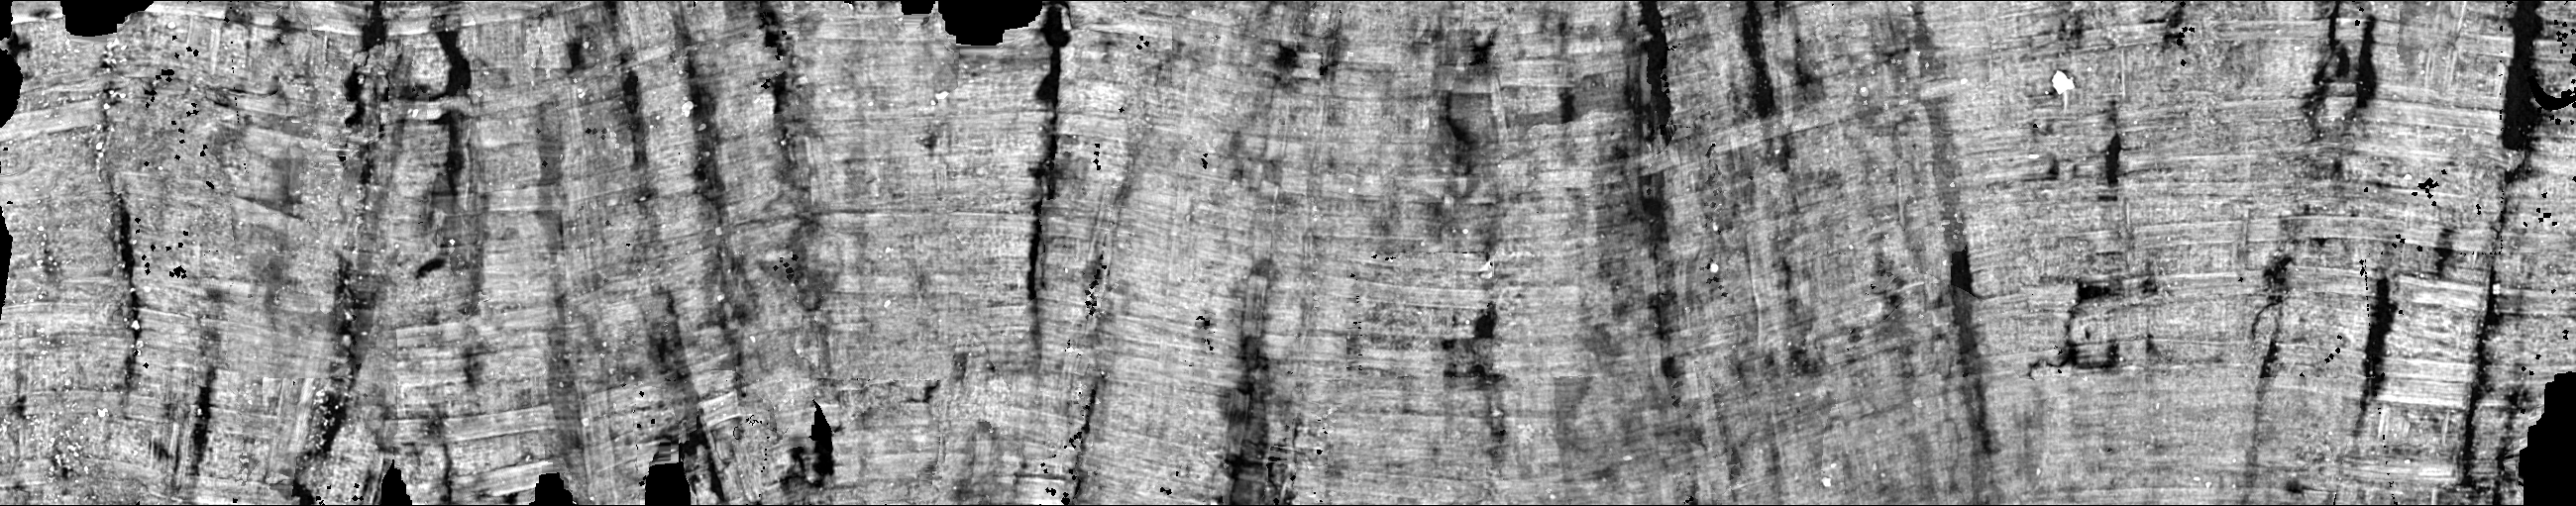
\includegraphics[width=\linewidth]{figures/unwrap_zoom.png}
  \caption{CT read-back from an accepted region of the developed $4\times5\times5$ experiment. The horizontal axis is developed arc length $u$ and the vertical axis is the scroll axis $v$. Continuous fibres and the perpendicular cross-hatch test the geometry and parameterization against the source volume; dark vertical bands are physical cracks and damage.}
  \Description{A wide grayscale developed CT texture with continuous fine fibre lines and several dark vertical crack bands.}
  \label{fig:unwrap}
\end{figure*}

